\section{Modelo}

% TODO: Agregar sobre la clasificación del problema (lo hago en la introducción ¿Borrar?)

% TODO: Señalar que aunque se habla de clientes pueden ser suministros, ¿Señalar aplicación en ubicación de plantas de biogas de papá?

Se tiene un conjunto de posibles ubicaciones para instalaciones $Z = \{z_1,z_2,...,z_{|Z|}\}$ y un conjunto ubicaciones de clientes $C = \{c_1,c_2,...,c_{|C|}\}$, cada cliente $c_i$ tiene asociado un peso o cantidad de demanda $w_i$.

Estas ubicaciones pueden ser vectores en $\mathbb{R}^N$, posiciones en una red o cualquier espacio métrico $\mathbb{E}$ en que se encuentre definida una métrica de distancia $d : \mathbb{E}^2 \rightarrow \mathbb{R}$ entre cada par de estas.

Se tiene el siguiente modelo de programación lineal:

\textbf{Índices:}
\begin{align*}
    i &= \text{índices de posibles clientes} \\
    j &= \text{índices de posibles ubicaciones de instalaciones} \\
    \text{\textbf{Inputs:}} \\
    w_i &= \text{Demanda del cliente $i$} \\
    \gamma &= \text{Costo fijo de colocar cada instalación} \\
    \alpha &= \text{Ganancia obtenida por cada unidad de demanda alcanzada} \\
    \beta &= \text{Costo de transportar una unidad de distancia una unidad de demanda} \\
    d_{ij} &= \text{Distancia entre cliente $i$ y la instalación $j$} = d(c_i,z_j)
\end{align*}

\textbf{Variables de decisión:}
\begin{align*}
    Y_{ij} &= \begin{cases}
        1 & \text{Si la demanda de $c_i$ es suplida por la instalación en $z_j$} \\
        0 & \text{Si no}
    \end{cases} \\
    X_{j} &= \begin{cases}
        1 & \text{Si se decide poner una instalación en $z_j$} \\
        0 & \text{Si no}
    \end{cases}
\end{align*}

\textbf{Maximizar:}
\begin{equation}
    - \sum_{j=1}^{|Z|} \gamma X_{j} + \sum_{i=1}^{|C|} \sum_{j=1}^{|Z|} \alpha w_i Y_{ij} - \sum_{i=1}^{|C|} \sum_{j=1}^{|Z|} \beta w_i d_{ij} Y_{ij}
\end{equation}

\textbf{Sujeto a:}
\begin{align*}
    Y_{ij} \leq X_{j} &\qquad \forall i \in \{1..|C|\} \quad \forall j \in \{1..|Z|\} \\
    \sum_{j=1}^{|Z|} Y_{ij} \leq 1 &\qquad \forall i \in \{1..|C|\} \\
    Y_{ij} = 0,1 &\qquad \forall i \in \{1..|C|\} \quad \forall j \in \{1..|Z|\} \\
    X_{j} = 0,1 &\qquad \forall j \in \{1..|Z|\}
\end{align*}

Este modelo corresponde a un caso particular de una de las variaciones mencionadas en \cite{mukundan1991joint}, en que los parámetros $d_{ij}$ cumplen con las propiedades de un espacio métrico, el costo de ubicar una instalación y la ganancia por alcanzar un cliente es independiente de su posición y el costo de transporte sólo depende de su nivel de demanda y su distancia.

\begin{figure}%
    \centering
    \subfloat[Ejemplo de un problema]{{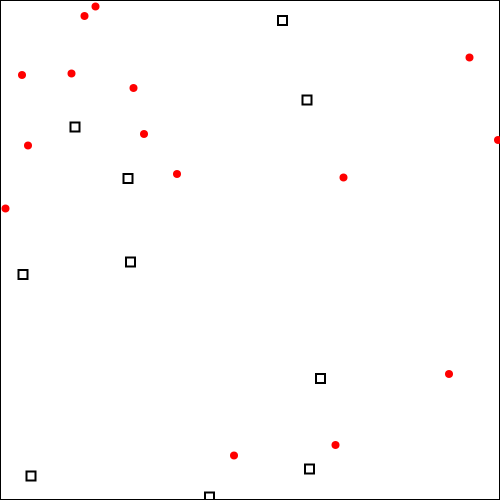
\includegraphics[width=5cm,height=5cm]{small_case_raw.png}}}
    \qquad \qquad \qquad
    \subfloat[Posible solución]{{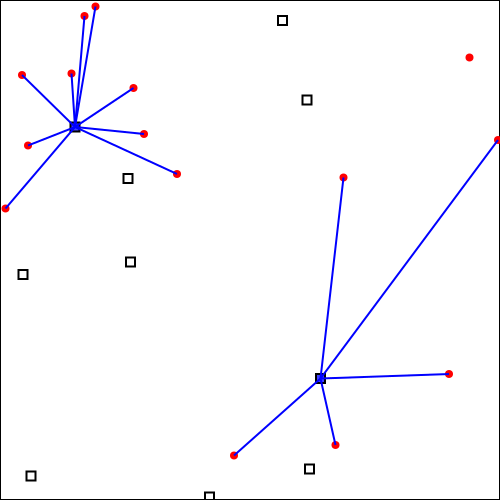
\includegraphics[width=5cm,height=5cm]{small_case_sol.png}}}
    \caption{A la izquierda, ejemplo de un problema, puntos rojos son ubicaciones de clientes, cuadrados son posibles ubicaciones de instalaciones.\\ A la derecha una posible solución, cuadrados azules representan subconjunto elegido de ubicaciones de instalaciones, clientes son trabajados por la instalación más cercana o ninguna si todas están muy lejos (tal es el caso del cliente en la esquina superior derecha).}
    \label{fig:problem}
\end{figure}

Notando que la función objetivo puede expresarse de la siguiente manera:
\begin{align*}
    -\sum_{j=1}^{|Z|} \gamma X_{j} + \sum_{i=1}^{|C|} w_i \sum_{j=1}^{|Z|} Y_{ij} (\alpha - \beta d_{ij})
\end{align*}

Es posible identificar un radio crítico $RC = \frac{\alpha}{\beta d_{ij}}$ pasado el cual no es conveniente suplir la demanda de un cliente. De la misma manera, puesto que la única variable controlable es $d_{ij}$, convendrá que la demanda de cliente sea suplida por la instalación colocada más cercana, a menos que esta se encuentre a una distancia mayor que el radio crítico.

La última observación permite expresar una solución al problema ya no como el conjunto de varibles de decisión $X_{j}$ y $Y_{ij}$, sino como un subconjunto $S$ de $Z$, buscando maximiziar el valor de la siguiente función objetivo $\Phi : \mathcal{P}(Z) \rightarrow \mathbb{R}$:

\begin{equation}
\Phi(S) = -\gamma \cdot |S| + \sum_{i=1}^{|C|} \max \left\{ 0 , \max_{z \in S} ( \alpha \cdot w_i - \beta \cdot w_i \cdot d(c_i,z)) \right\}
\end{equation}

Una solución $S$ se traduce a una solución para el modelo de programación lineal, asumiendo por simplicidad y sin pérdida de generalidad que las distancias $d_{ij}$ son diferentes, de la siguiente manera:

\begin{align*}
    X_{j} &= \begin{cases}
        1 &\quad z_j \in S \\
        0 &\quad z_j \notin S
    \end{cases}\\
    Y_{ij} &= \begin{cases}
        1 &\quad (d_{ij} \leq RC) \wedge (d_{ij} \leq d_{ik} \quad \forall k : z_k \in S)
        \\
        0 &\quad e.o.c.
    \end{cases}
\end{align*}

Siendo las soluciones generadas de esta manera siempre igual o mejores que sus contrapartes con distintos valores $Y_{ij}$, se reduce el espacio de búsqueda, a uno con soluciones descritas completamente por un subconjunto de instalaciones elegido.

% TODO: U N D E R S T A N D
% Una propiedad que vale la pena destacar es que si se tiene una solución $P$ y una instalación $q$:
% \begin{equation}
%     \Phi(P) > \Phi(P \cup \{q\}) \wedge (P \subseteq R) \RightArrow  \Phi(R) > \Phi(R \cup \{q\})
% \end{equation}

\section{Algoritmo}

El algoritmo comienza encontrando todas las ubicaciones de instalaciones que, por si solas, tienen función objetivo positiva:
\begin{equation}
G = \{ s |  \quad s \in Z, \quad \Phi(\{s\}) \geq 0 \}
\end{equation}
Estas ubicaciones forman la \emph{base} de soluciones de tamaño 1:
\begin{equation}
B_1 = \{ \{g\} | \quad g \in G \}
\end{equation}

El algoritmo procede realizando iteraciones, cada una consiste en un proceso de \textbf{reducción} de la base a una cantidad manejable de soluciones representativas (llámese \emph{pool}) y una posterior \textbf{expansión} de esta \emph{pool} para formar la \emph{base} de soluciones de tamaño mayor.

El proceso de reducción se puede escribir como:
\begin{equation}
P_n = Reduce(B_n)
\end{equation}
donde la función $Reduce$ se explicará más adelante. El algoritmo trabaja con un parámetro \texttt{POOL\_SIZE} que indica la cantidad máxima de soluciones que puede tener una \emph{pool}, una mayor \emph{pool} explorará más posibles soluciones pero tendrá un costo computacional mayor.

Por otro lado el proceso de expansión está dado por:
\begin{equation}
B_{n+1} = \{S = p \cup \{g\} |
    \quad p \in P_n, \quad g \in G, g \notin P_n, \forall (p \in P_n)( p \not\subset S \vee \Phi(p) < \Phi(S)) \}
\end{equation}
Este consiste en tomar cada solución de la \emph{pool} y agregarle una nueva instalación de $G$ de todas las formas posibles que aumenten el valor de la función objetivo. Nótese que una solución nueva puede ser generada a partir de más de una solución en la \emph{pool}, pero para que esté en la siguiente \emph{base} debe tener una mejor ganancia que todas las soluciones que pueden generarla dentro de la \emph{pool}, puesto que de otra manera sería seguro que, para esta solución y todas las soluciones de las que sea subconjunto, existirá una instalación que al removerla, aumentará el valor de la función objetivo.

% TODO: Explain more? ^

También es importante notar que tanto en la base $B_i$ como en la pool $P_i$ todas las soluciones son de tamaño $i$.


% TODO: U N D E R S T A N D
% Una solución con una instalación inútil, generada a partir de una solución $p$, i.e. que al sacarla el valor de la función objetivo no disminuye, no dejará de serlo en soluciones en que $p$ sea un subconjunto, por la propiedad de \emph{no-sinergia} por lo que dichas soluciones no son de interés, por la misma razón $g$ itera sobre $G$ y no $Z$.


El algoritmo termina cuando la base de la generación siguiente se encuentra \emph{vacía}, y retorna la combinación $\hat{S}$ que haya logrado un mayor valor de la función objetivo $\Phi$ de entre todas las \emph{pools} $P_i$.
